\PassOptionsToPackage{dvipsnames}{xcolor}
\documentclass[twocolumn, twocolappendix]{aastex631}
% \received{\today}
\shorttitle{RATRATARRATRATTS}
\graphicspath{{figures/}}

\usepackage{lipsum}
\usepackage{physics}
\usepackage{multirow}
\usepackage{xspace}
\usepackage{natbib}
\usepackage{fontawesome5}
\usepackage{xcolor}
\usepackage{wrapfig}
\usepackage[figuresright]{rotating}

% remove indents in footnotes
\usepackage[hang,flushmargin]{footmisc} 

\usepackage{styles/todo_notes}

\newcommand{\placeholder}[1]{{\color{gray} \lipsum[#1]}}

% custom function for adding units
\makeatletter
\newcommand{\unit}[1]{%
    \,\mathrm{#1}\checknextarg}
\newcommand{\checknextarg}{\@ifnextchar\bgroup{\gobblenextarg}{}}
\newcommand{\gobblenextarg}[1]{\,\mathrm{#1}\@ifnextchar\bgroup{\gobblenextarg}{}}
\makeatother

\newcommand{\tauriRAT}{RATTS\xspace}
\newcommand{\radioRAT}{RRAT\xspace}
\newcommand{\binaryRAT}{RRATRATTS\xspace}

\newcommand{\rebound}{\texttt{REBOUND}\xspace}
\newcommand{\cosmic}{\texttt{COSMIC}\xspace}
\newcommand{\cogsworth}{\texttt{cogsworth}\xspace}

\newcommand{\hi}[1]{{\color{gray} #1}}

\definecolor{dark}{rgb}{0.2,0.2,0.2}
\newcommand{\darkmode}{
    \pagecolor{dark}
    \color{white}
    \hypersetup{linkcolor=yellow,urlcolor=yellow,
                anchorcolor=yellow,citecolor=yellow}
}

\begin{document}

% \darkmode{}

\title{{\Large RATRATARRATRATTS}\\ir\hi{R}adi\hi{AT}ed \hi{rat}s \hi{A}round \hi{R}otating \hi{RA}dio \hi{T}ransients \hi{R}evolving \hi{A}bout \hi{T}he \hi{R}un\hi{A}way \hi{T}-\hi{T}auri \hi{S}tar}

% affiliations
\newcommand{\UW}{Department of Astronomy, University of Washington, Seattle, WA, 98195}

\author[0000-0001-6147-5761]{Tom Wagg}
\affiliation{\UW}

\author[0000-0003-0484-3331]{Andy Tzanidakis}
\affiliation{\UW}

\author[0000-0002-3221-9395]{V Hurtado}
\affiliation{\UW}

% \author{...you?}
% \affiliation{\UW}

\correspondingauthor{Tom Wagg}
\email{tomjwagg@gmail.com}

\begin{abstract}
    Astronomers have pondered the nature of Rotating RAdio Transients (\radioRAT{}). They have scrutunised the RunAway T-Tauri Stars (\tauriRAT{}). But never before have they considered \radioRAT{}s \textit{revolving about} \tauriRAT{}s (\binaryRAT). In this interdisciplinary paper, we investigate formation mechanisms for \binaryRAT{}s and the prospect of detecting irradiated rats on planets around them.

    %Neutron stars that undergo electron-capture supernovae are thought to experience weaker kicks (on the order of $30 \unit{km}{s^{-1}}$) resulting in velocities similar to ejected T-Tauri stars.
    A pulsar-main sequence binary propelled by a supernova natal kick in the vicinity of a star forming region may encounter a \tauriRAT{}. Using N-body simulations we demonstRATe that a dynamical three-body encounter between these objects could lead to the ejection of the main sequence and the formation of a \binaryRAT{}. Our expert astrobiologists consider the level of irradiation that a planet in the system would experience from a combination of the pulsar beams and the activity from the T-Tauri star. We consider how a highly specialised species of rat may evolve to survive these conditions. Finally, we ponder the ubiquitous and fundamental nature of the concept of rats in the Universe.
\end{abstract}

\keywords{April Fools, Rats, \tauriRAT{}s, \radioRAT{}s, \binaryRAT{}s, The Joy of Acronyms}

% \tableofcontents

% \Large

\section{Introduction}
Rats. For many, that word brings to mind a scurrilous, unkempt little rodent, prowling the streets of their favourite city. But not astronomers. No, they looked beyond this simple view and thought to ask the question: what more could a rat be?

Why of course, they stated, a rat could be a runaway T-Tauri star (\tauriRAT, \citealp{Sterzik+1995}), a young protostar, heartlessly ejected from its parent molecular cloud, set free into the depths of space! Later, others cried that a rat could be a rotating radio transient (\radioRAT, \citealp{McLaughlin+2006}), a rapidly spinning neutron star (NS) living as a remnant of its former self, emitting momentary radio bursts.

And now, at last, with this paper we contemplate how these rats may come together as a Rotating Radio Transient Revolving About The RunAway T-Tauri Star (\binaryRAT).% In this way they may breathe life back into one another, as well as newly formed nearby planets, spurring on the creation of yet another form of rats.

% \subsection{Recent \tauriRAT{} observatio\textbf{}ns}
Until recently, few \tauriRAT candidates have been observed \citep[e.g.][]{Neuhauser+1996,Neuhaeuser+1997}. But with the discovery of UJT-1 in \citet{Marti+2023}, this class of object has been revived. The \tauriRAT was first proposed as an explanation for finding infant stars, isolated from their parent molecular clouds \citep{Sterzik+1995, Sterzik+1995b}. Their isolation is a thought to be a result of few-body interactions between young multiple star systems in the core of collapsing molecular clouds.

% \subsection{Known sample of \radioRAT{}s}
In contrast, there are more than a hundred known \radioRAT{}s, as recorded in the RRATCat \citep{RRATCat} and RRATalog\footnote{Though both names are excellent, we do highlight that the RRATalog avoids mentioning cats, which could help to avoid scaring off other \radioRAT{}s in future surveys...} \citep{RRATalog}. Despite their relative abundance, these \radioRAT{} are still viewed as ``mysterious'' \citep[e.g.][]{mysterious_RRAT}, with many potential explanations for their millisecond long bursts of radio activity.

% \subsection{The confusion between \tauriRAT{}s and \radioRAT{}s}
Some might argue that the acronyms assigned to the noble \tauriRAT and \radioRAT objects are overly similar, confusing even, for the uninitiated reader. On the contrary we emphasise that the confusion you may feel is but a symptom of the awe engendered by the fundamental nature of rats in the Universe. We will elaborate further on this realisation in Section~\ref{sec:fundamental_rats}.

% \subsection{This paper and the \binaryRAT}
In this paper we bring together two disparate\footnote{dispaRATe? Conincidence? I think not.} classes of objects and consider what one could achieve through their union as a \binaryRAT. In Section~\ref{sec:rat_formation} we discuss and demonstrate a potential formation mechanism for \binaryRAT{}s. In Section~\ref{sec:radiation} we consider the radiation that a planet in a \binaryRAT system may be subjected to, and thus in what ways rats may need to evolve. We delve further into the philosophy of the fundamental nature of rats in our Universe in Section~\ref{sec:fundamental_rats} and finally draw our conclusions.

\section{\binaryRAT{} formation}\label{sec:rat_formation}

The formation of a \binaryRAT system in-situ (i.e.\ formed as a binary) may prove difficult given the dramatic nature of dynamical encounters necessary to eject a \tauriRAT from a molecular cloud (see Section~\ref{sec:tts_ejections}). We therefore postulate that a \binaryRAT may be formed \textit{dynamically}, through a 3-body encounter between a \tauriRAT and a binary containing a \radioRAT. In the following subsections we explain how each of these systems can acquire the requisite velocity and demonstrate how such an encounter might proceed.

\subsection{Evolving a \radioRAT--MS binary}

In this Section, we explain how one might go about forming a \radioRAT in a binary with a main sequence (MS) star. Given exact nature of the \radioRAT is not currently known (and that it makes my life a lot easier), we make the simplifying assumption that every NS is a \radioRAT.

We use the rapid binary population synthesis code \cosmic \citep{COSMIC} to simulate example evolution of a \radioRAT--MS system. We drew binaries using the \cosmic default settings and rapidly evolved them until we found a bound NS--MS binary. Using \cogsworth, we automatically converted the evolution table outputted by \cosmic into the cartoon evolution shown in Figure~\ref{fig:cartoon_ms_ns}. \tom{Come back and actually describe this evolution once I decide if this is a good example}

We highlight that the natal kick magnitude that a NS receives upon supernova is likely much smaller in the case of electron-capture supernovae \citep[e.g.][]{Miyaji+1980, Gessner+2018, Igoshev+2020}, on the order of $30 \unit{km}{s^{-1}}$. These lower kick decreases the chance of binary disruption and means that a \radioRAT--MS binary would approach a \tauriRAT-forming molecular cloud at a lower velocity, allowing for more effective 3-body encounters.

\begin{figure}
    \centering
    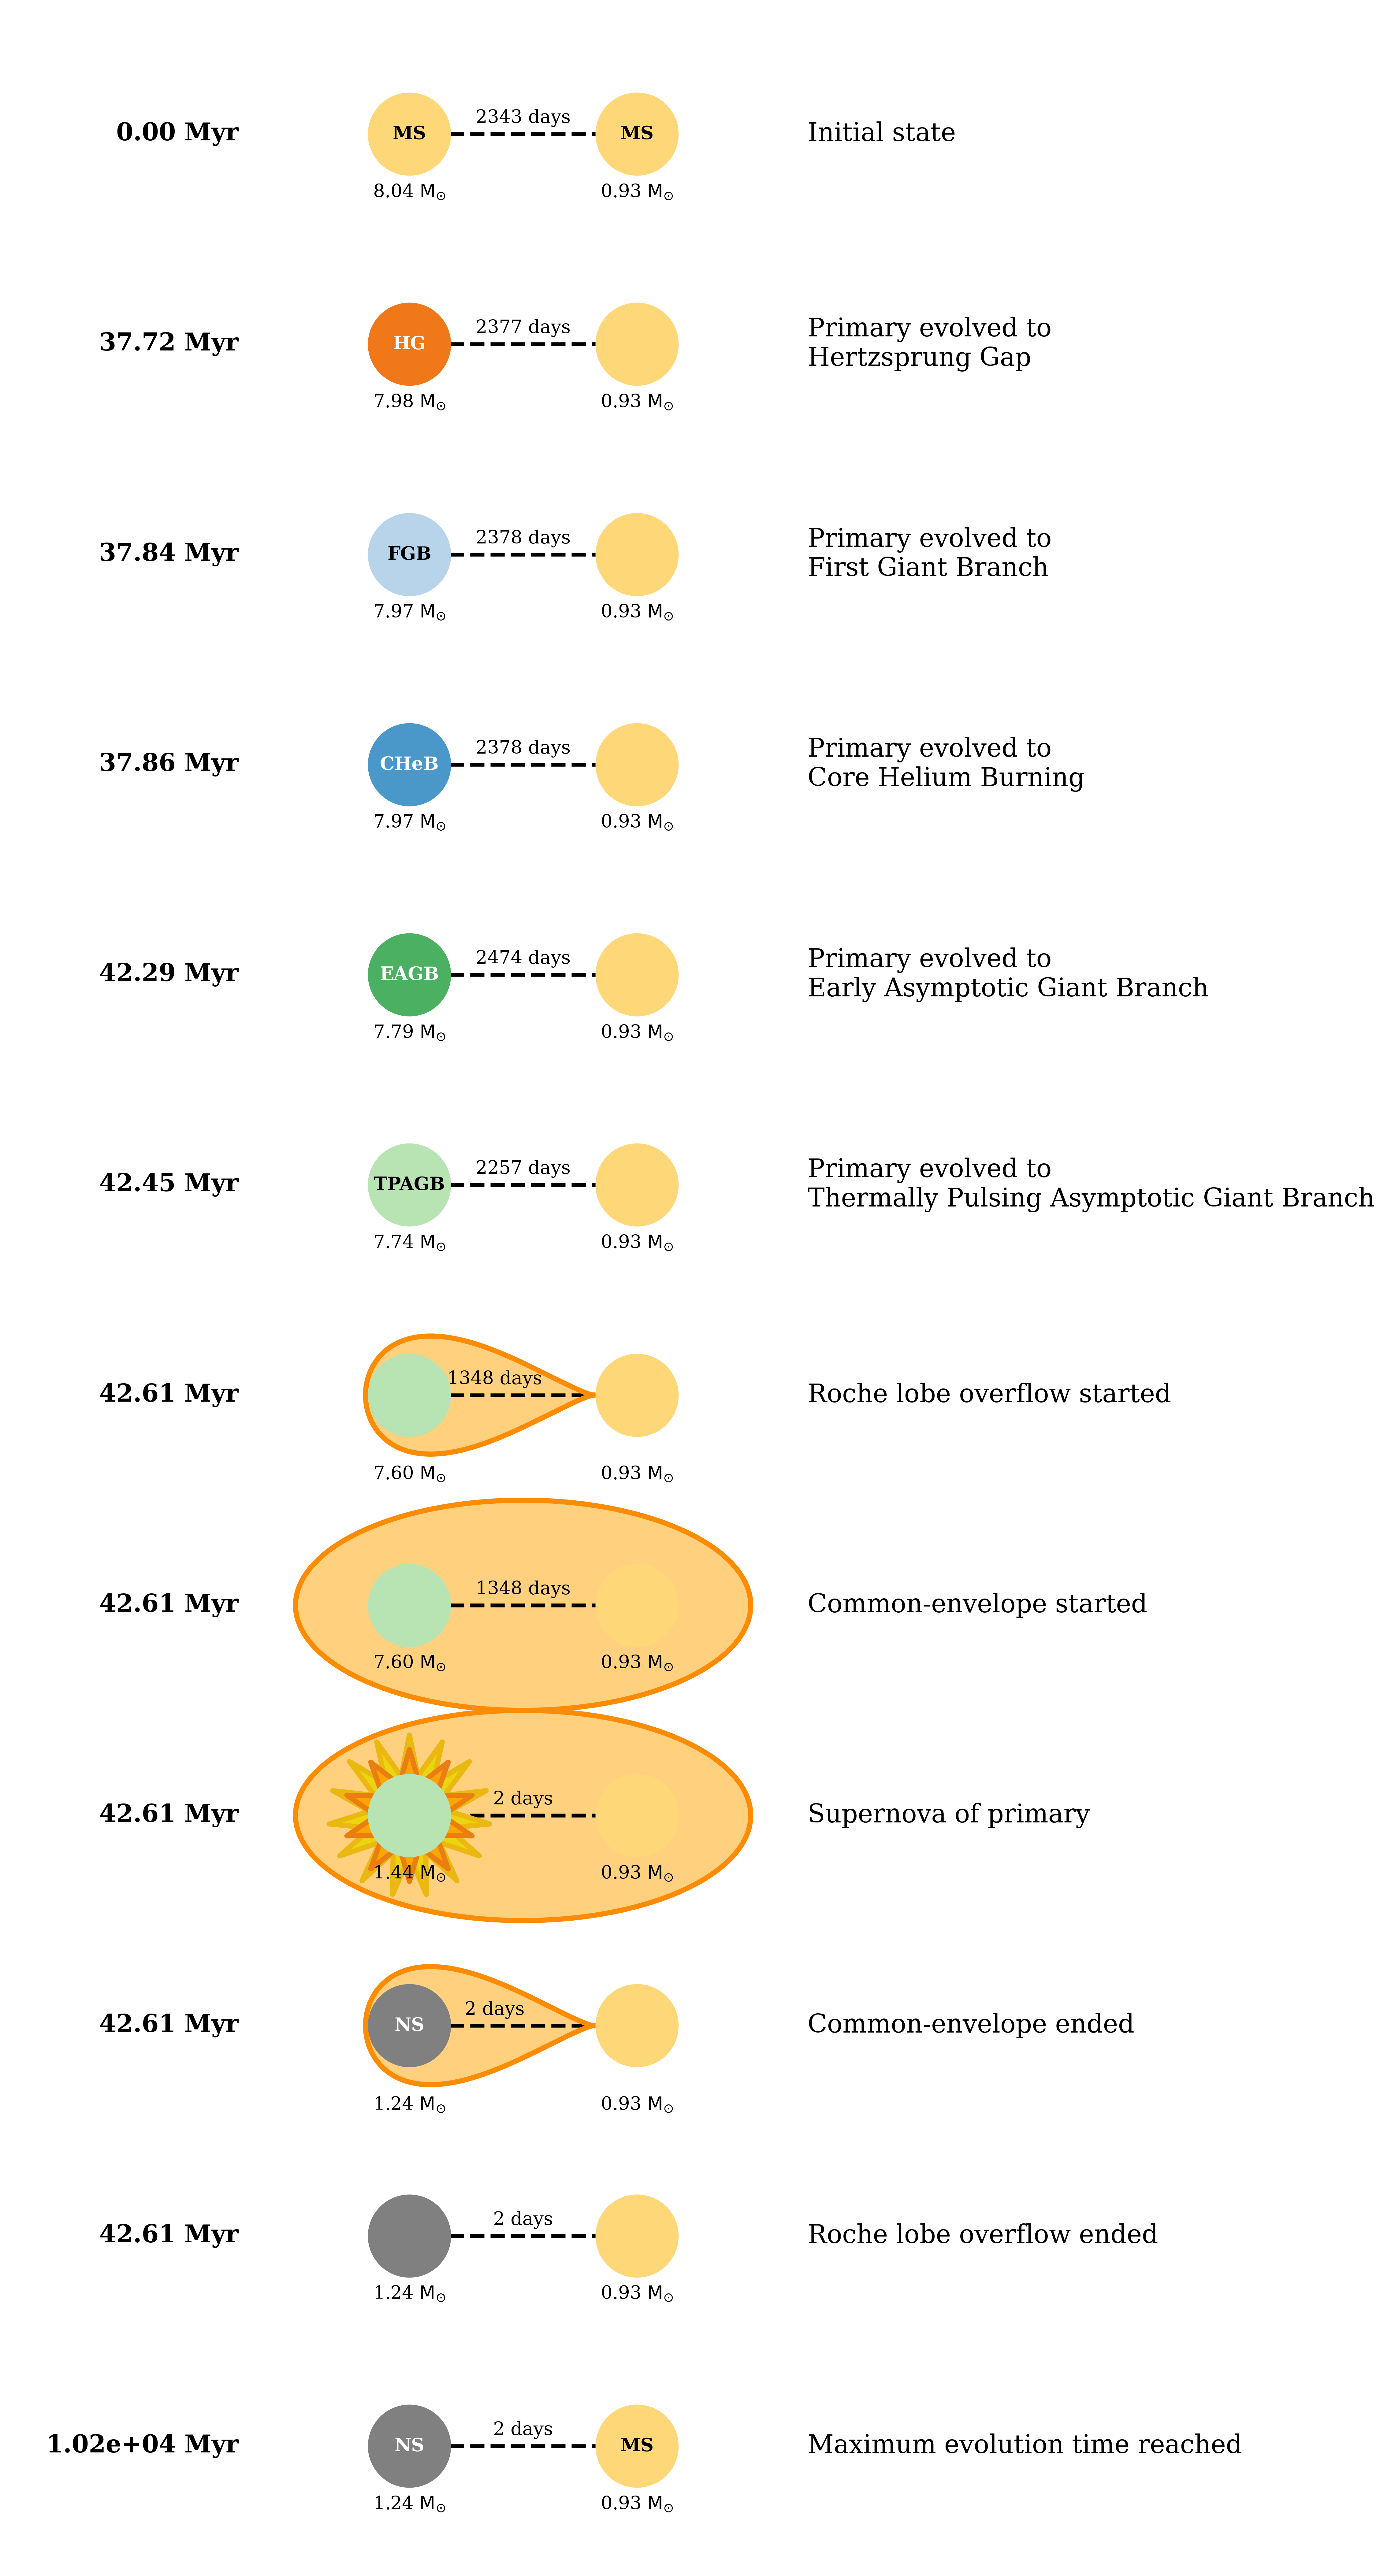
\includegraphics[width=\columnwidth]{figures/cartoon.png}
    \caption{Example evolution of a neutron star--main sequence binary through the common-envelope channel, simulated with \cosmic. Automated visualisation achieved with \cogsworth. Each row is row represents a different evolutionary stage and is annotated with the masses of each star, orbital period and stellar type where applicable.}
    \label{fig:cartoon_ms_ns}
\end{figure}

\subsection{T-Tauri ejections from molecular clouds}\label{sec:tts_ejections}

\tom{Explain how dynamical encounters can ejects stars from clouds}

\subsection{N-body simulations of \binaryRAT{}s}

\begin{figure}[htb]
    \centering
    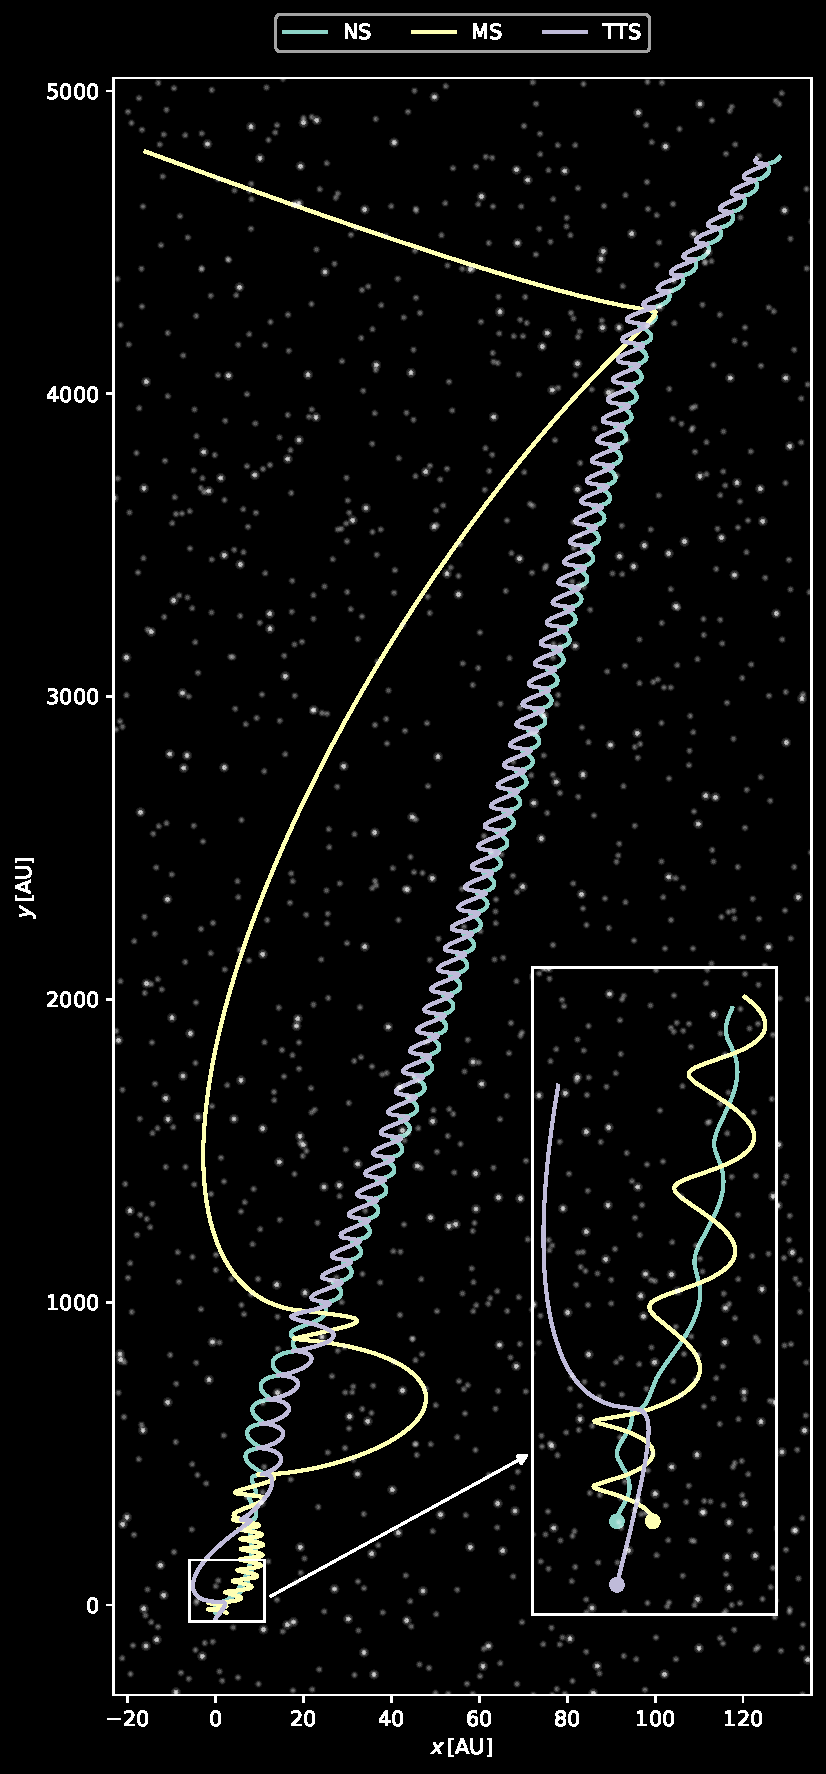
\includegraphics[width=\columnwidth]{rat_formation.pdf}
    \caption{An example formation scenario of a \binaryRAT through a 3-body exchange process between a \tauriRAT and a binary containing a main sequence star and a \radioRAT. Inset panel shows the detail of the initial evolution (with scatter points to highlight staring positions). An animated version of this plot is available \href{https://www.tomwagg.com}{here}.\\\textbf{NOTE:} Of critical importance, upon rotating the image to the right (and squinting heavily), the outline of a rat is revealed (\href{https://www.tomwagg.com}{see here} for an annotated version)!}
    \label{fig:rat_rebounding}
\end{figure}

We use the N-body code \rebound\citep{REBOUND} to simulate a 3-body encounter between a \tauriRAT and a binary containing a \radioRAT and a main sequence star. We initialise a binary containing a $1.4 \unit{M_\odot}$ neutron star and $0.3 \unit{M_\odot}$ main sequence star with an orbital separation of $2.5 \unit{AU}$, moving with a centre of mass velocity of approximately $30 \unit{km}{s^{-1}}$ (motivated by the assumption that the NS underwent an ECSN). We then add a \tauriRAT of mass $0.9 \unit{M_\odot}$, moving with a velocity of approximately $45 \unit{km}{s^{-1}}$ towards the binary and trace the evolution of the system.

We show the evolution of this system in Figure~\ref{fig:rat_rebounding}. The interaction between the \tauriRAT and initial binary leads to a series of several chaotic encounters, at the end of which the main sequence star is ejected and a \binaryRAT system is formed.

\section{Radiation and Rat Evolution}\label{sec:radiation}
\subsection{Radiation in the vicinity of a \binaryRAT}
\todo{Estimate the radiation one might expect when orbiting a \binaryRAT, considering both components - jet emission from rotating NS? Periodic outbursts from a TTS?}

\subsection{Terrestrial examples of specialised rat evolution}
\andy{Andy wants to write this subsection}
Rats have already demonstrated a remarkable ability to adapt to their environments through specialised evolution. Let us consider some terrestrial examples of this sort of evolution:
\begin{itemize}
    \item NYC Pizza Rat
\end{itemize}
Beyond these examples, human imagination knows no bounds in considering other forms of potential rat evolution
\begin{itemize}
    \item Remy from Ratatouille
    \item Splinter from TMNT
    \item Rattata
    \item Scabbers a.k.a Peter Pettigrew
\end{itemize}

\missingfigure{Grid of faces of famous rats?}

\section{The fundamental nature of rats}\label{sec:fundamental_rats}
\v{v has thoughts here}
\begin{itemize}
    \item In many ways, albeit primarily orthographically, rats are simply a reflection of a star and thus it is no surprise astronomer are drawn to acronyms involving them
    \item Scientists across astronomy, gastronomy, biology discover, classify and invent rats
    \item Rats are present in the case of baby stars (\tauriRAT), regular stars (regular rats) and dead stars (\radioRAT), thus spanning the entire life of stars
\end{itemize}


\section*{Conclusions}%\label{sec:conclusions}
In this paper, we present new findings relating to \binaryRAT systems and their potential to host planets supporting life for irradiated rats. Though our conclusions are many and far reaching, we leave you with some of the main implications of this work:
\begin{enumerate}
    \item \textbf{Astronomers love rats}\\Whether they are running away, rotating rapidly or simply roaming the streets, astronomers cannot stop name objects after rats.
    \item \textbf{The acronyms have gone too far folks}\\It may be time for astronomers to accept that the acronyms, and in particular back-ronyms\footnote{\url{https://en.wikipedia.org/wiki/Backronym}} are getting a little out of hand.
    \item \textbf{I should really go and work on my thesis}\\Sleep deprivation and procrastination make for powerful creative writing aids, except in the case of a thesis.
\end{enumerate}

\software{\rebound \citep{REBOUND}, \cosmic \citep{COSMIC}, \cogsworth, Python \citep{python}, \texttt{matplotlib} \citep{matplotlib}, \texttt{numpy} \citep{numpy} }

\begin{acknowledgements}
    We are deeply grateful to Eric Agol for bringing the concept of a \radioRAT{} to our attention during a journal club presentation on \tauriRAT{} by Tom Wagg - without this critical input our insightful work might never have been realised.
\end{acknowledgements}

\bibliography{bibs/software.bib, bibs/paper.bib}

\appendix
\section*{A story of further evidence}
\todo{Write out a whole paragraph where each first letter of the line spells out some message about rats - more fun if it is a story about us}

How might this all relate to rats you ask? Try reading vertically instead of horizontally and see what fundamental message on rats that you uncover.

\end{document}